
% introduction of vms 
\subsection{Virtualisation}
To resolve this problem, practitioners tend to use Virtualisation. Using virtual machines aka VM gives reaserchers the freedom to choose their own tools, software and operating system that they are the most confortable with without paying the price to change the actual working environment, which will give them eventually more controle over the dependencies and the execution environement. Moreover, using a vm will solve the \emph{replication crisis} thanks to the virtual images, even the most complex architecture can be reproduced easily by just instantiating a copy of the image. Since the virtual machines are agnostic to the host architecture, reaserchers won't have to worry about where and how their experiments are replicated because they have already setup the execution environement. Another advantage to the virtual machines is the snapshot mechanism, it allows reaserchers to create backups and revert some changes with simple clicks. Last but not least,thanks to the isolation, virtual machines push the reproducibility further by allowing the future usages to see all the variables -controled and uncontroled-  and do other analysis without dealing with any dependencies. In his paper \cite{howe_virtual_2012} bill howe lists the advantages of using virtual machines in reaserchers experements including the economical impact and cultural limitation to a such approach.

which allow them to have control over the ressouces, the dependencies and the execution environment. Moreover, thanks to the snapshots, deploying a software is easily done by instantiating a copy of that image.
However, this choice comes with a certain cost. Because the intervention of the hypervisor,the software will use two kernels , the virtual machine one and the host machine one, which will provide a noticiable overhead, and will impact the performances of the tests.Therefore, we can't use virtual machines for exepements that are related to performance. Another limiation with the virtual machine is the the isolation. It is true that this feature will prevent the experience environement with any undesirable interference from the outside world. but sometimes this contact is needed, especially when the experiment is dependent to an external part, such as sensors. In energicial tests we tend to use hardware powermeters which will make it difficult to use the virtual machines in this case .

% introduction of docker 

\begin{figure}
    \center{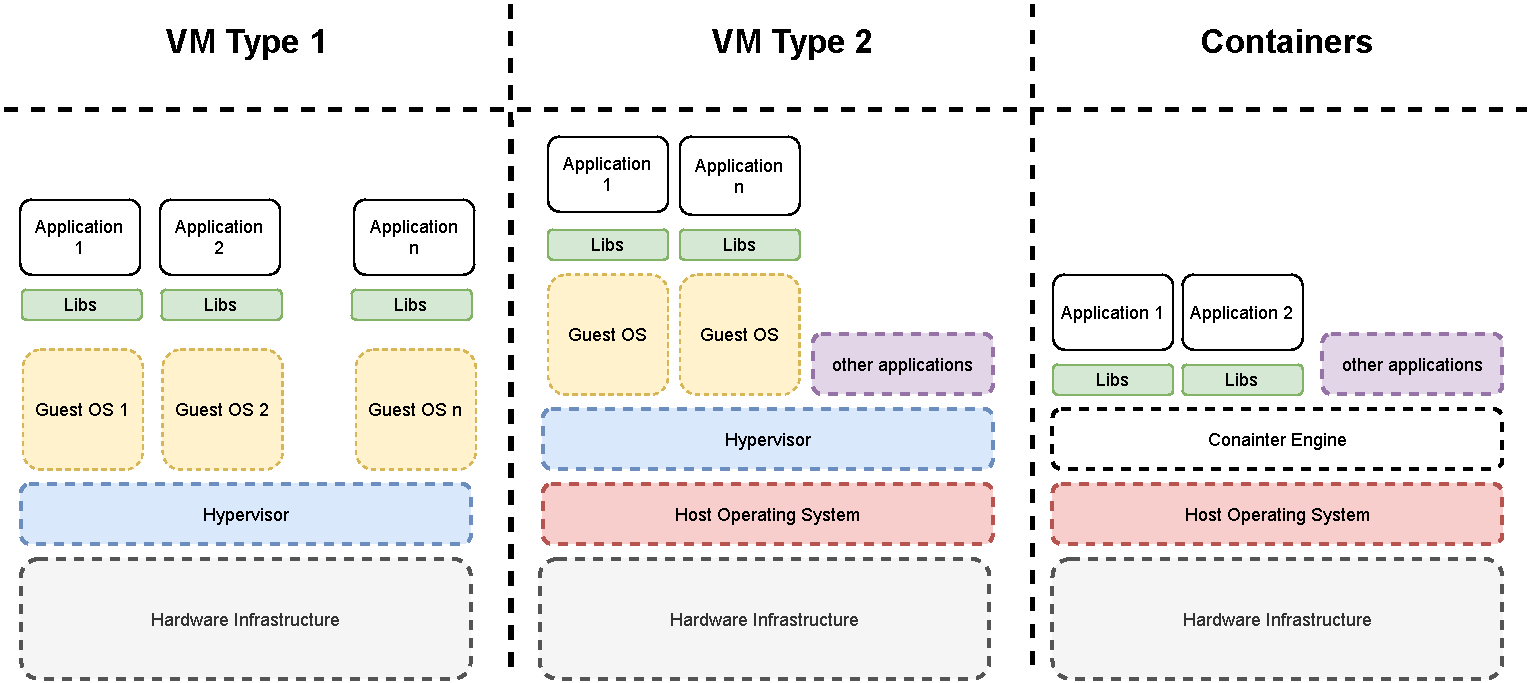
\includegraphics[width=1\linewidth]{imgs/virtualization_techniques}}
    \caption{Different Methods of Virtualzation}\label{environement:virtualization_technique}
\end{figure}

\subsection{Containers}

another solution would be using something that allows us to have the isolation from the host os and the ease of replication that virtual machines offer, and the direct interaction with the hardware that the classical method give.
contarization offers a such advantages while keeping the isolation and the ease of replication for application.

Figure \ref{environement:virtualization_technique} explains the differents in architecture between the clasic types2 of Virtualisation and Containers.
\begin{itemize}
    \item Type 1: runs directly on the hardware, it is mainly used by the cloud providers where there is no main OS, but just virtaul machines, we can site for this the open-srouce XEN and VMware ESX
    \item Type 2: runs over the hostmachine Operating System, mostly used for personal comptuers, VMware server and virtualBox are famous examples of this type, most of the reaserchers expermentation are run witht this type, howerver due to the 2 Operatings syestms the applications tend to be more slower
    \item containers : Instead of its own kernel, containers used the hots kernel to run their Os, which makes them ligher, quickers and use the full pontial use of the hardware. For this we can cite \emph{Docker}, \emph{Linux LXC}\emph{LXD} \cite{abuabdo_virtualization_2019}
\end{itemize}
%  TODO Rephrase so i include it before VMs+ add links to the technologie


\subsection{Docker vs Virtual Machine}
Depsite that Type 1 is more performant than type 2, the second one is the most used in reaserch, since most researchers conducts their experements in their own machine. In the other hand, docker is the most famous thechonology for for containers.
In ower case we are more prone to docker for two reasons.
\begin{enumerate}
    \item we need a litetweight orchestrator to not affect the energy consumption of ower tests. As prior work mentioned [cite Morabito (2015) and van Kessel et al. (2016)]
          % cite Power efficiency of hypervisor-based virtuali- zation versus container-based virtualization. University of Amsterdam.
    \item since we are using the hardware itself to measure the energy consumption, we are required to interract with the host OS itself.
\end{enumerate}
Special notice to \href{https://github.com/powerapi-ng/virtualwatts}{virtualwatts}. A framework that allows us to retireve the energy consumption of a virtual machine.
%%%%% THINGS TO ADD : 
%% -------------- Dont think so 
% the impact of docker on the reprodudicibility 
% Limits of docker 
% The docker files and the clarification of the methodology 
\subsection{Docker and energy}
Now that we have chosen to go with the containers technorolgy to encapsulate our tests. What would be the impact of this solution on the energy consumption of our tests.

Based on the studies of \cite{santos2018does}, who analysed the impact of adding the docker layer on the energy consumption.
In their experement. Eddie Antonio et al run multiple benchmarks with and without docker. and compared their energy consumption and execution time.
The first step was to see the impact of docker deamon while there is no work. to see the impact of the orchestrator alone. Later they had the experiment with the following benchmarks
\begin{itemize}
    \item wordpress
    \item reddis
    \item postfresSQL
\end{itemize}
The following figures represents the energy consumption of the system while it is idle. As we can see  in figure \ref{fig:docker_idle} Docker braught arround 1000joules overhead.
\begin{figure}
    \center{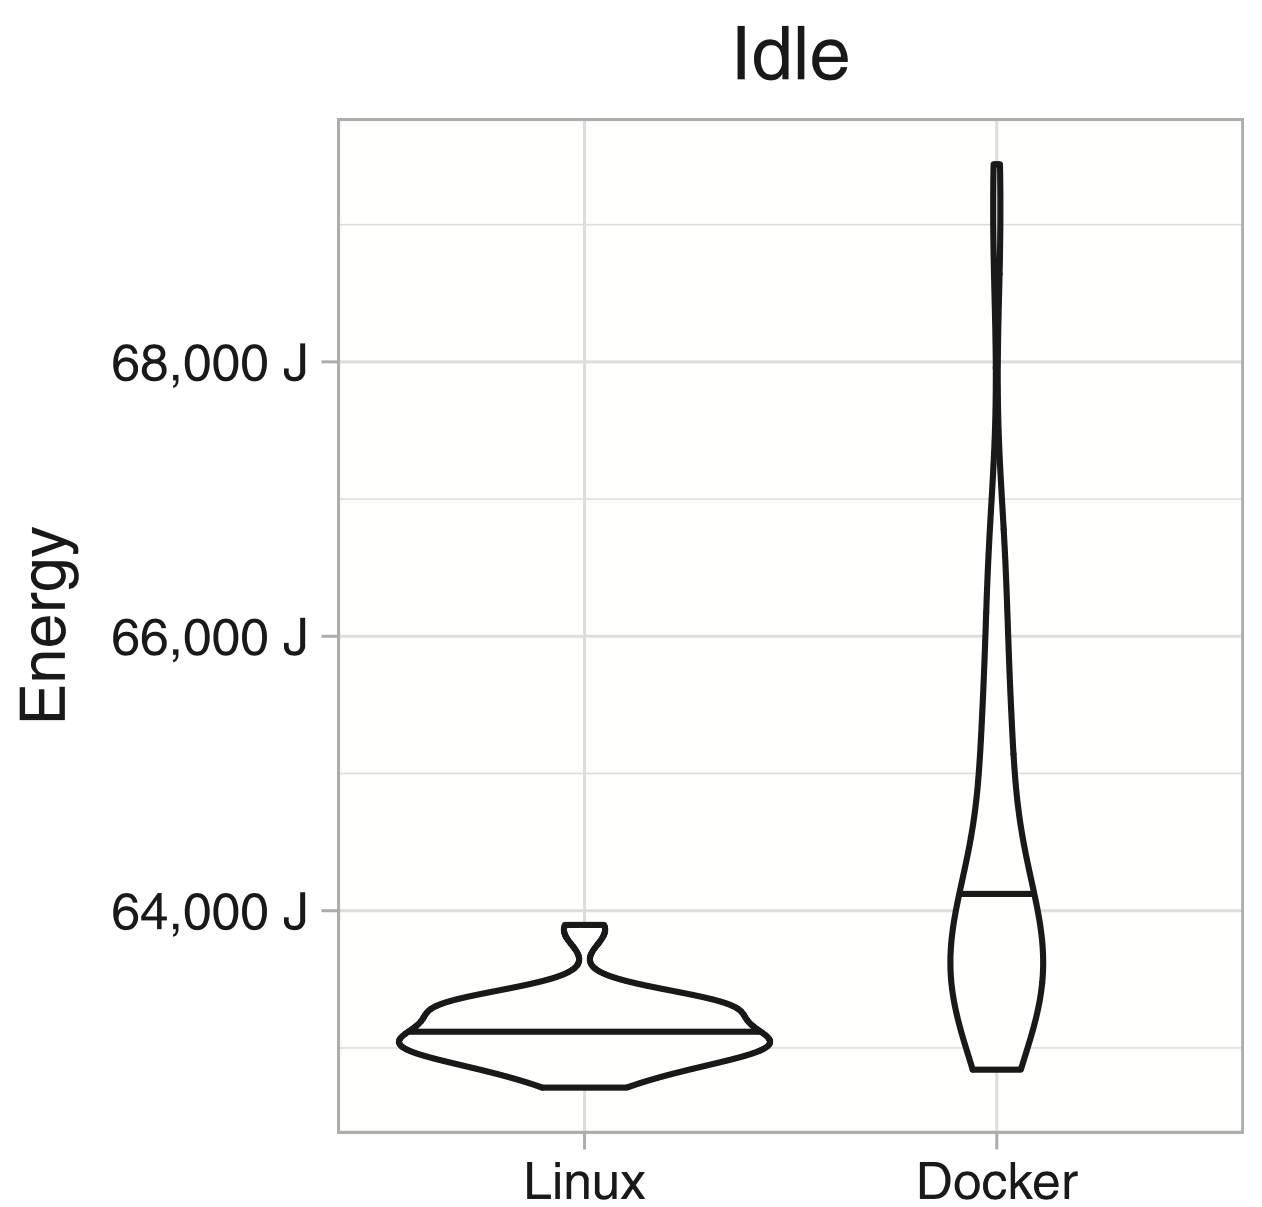
\includegraphics[width=.5\linewidth]{imgs/docker_vs_vm_energy_paper/idle_energy}}
    \caption{energy consumption of Idle system with and without docker \cite{santos2018does}}\label{fig:docker_idle}
\end{figure}
In the other hand as we can see in figure \ref{fig:docker_reddis}. docker increased the execution time of the benchmark by 50 seconds which caused an increase in energy since they are highly correlated.
The authors also highlated the fact that this increase of energy consumption is due to the docker deamon and not the fact that the application is in a container. Moreover they estimted the price of this extra energy and it was less than 0.15\$ in the worst case. Which is non significant compared to the advantages that docker bring for isolation and reproducibility.\\
if we  recap this study in one sentence,it would be the following one.
The dockerised softwares tend to consume more energy, because mainly they take more time to be executed.
The average power consumption is higher with only \textbf{2Watts} and it is due to the docker deamon.This overhead can be up to 5\% for IO intensive application, but it is mearly noticiable when it comes to CPU or DRMA intesive works



\begin{figure}
    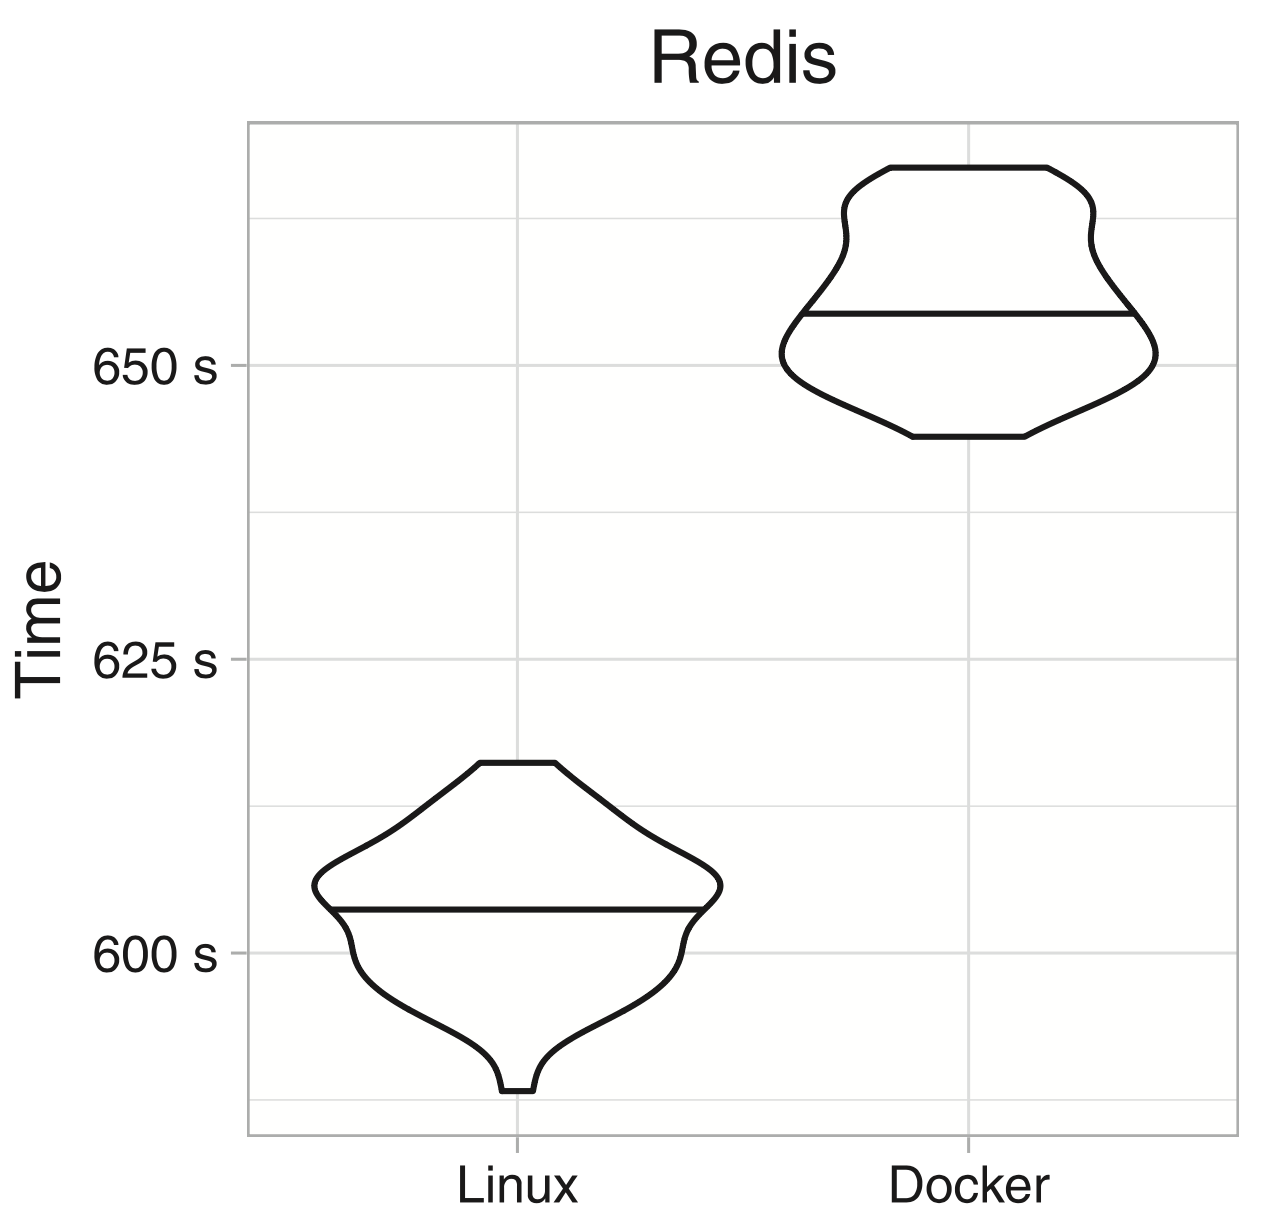
\includegraphics[width=.5\linewidth]{imgs/docker_vs_vm_energy_paper/reddis_time}
    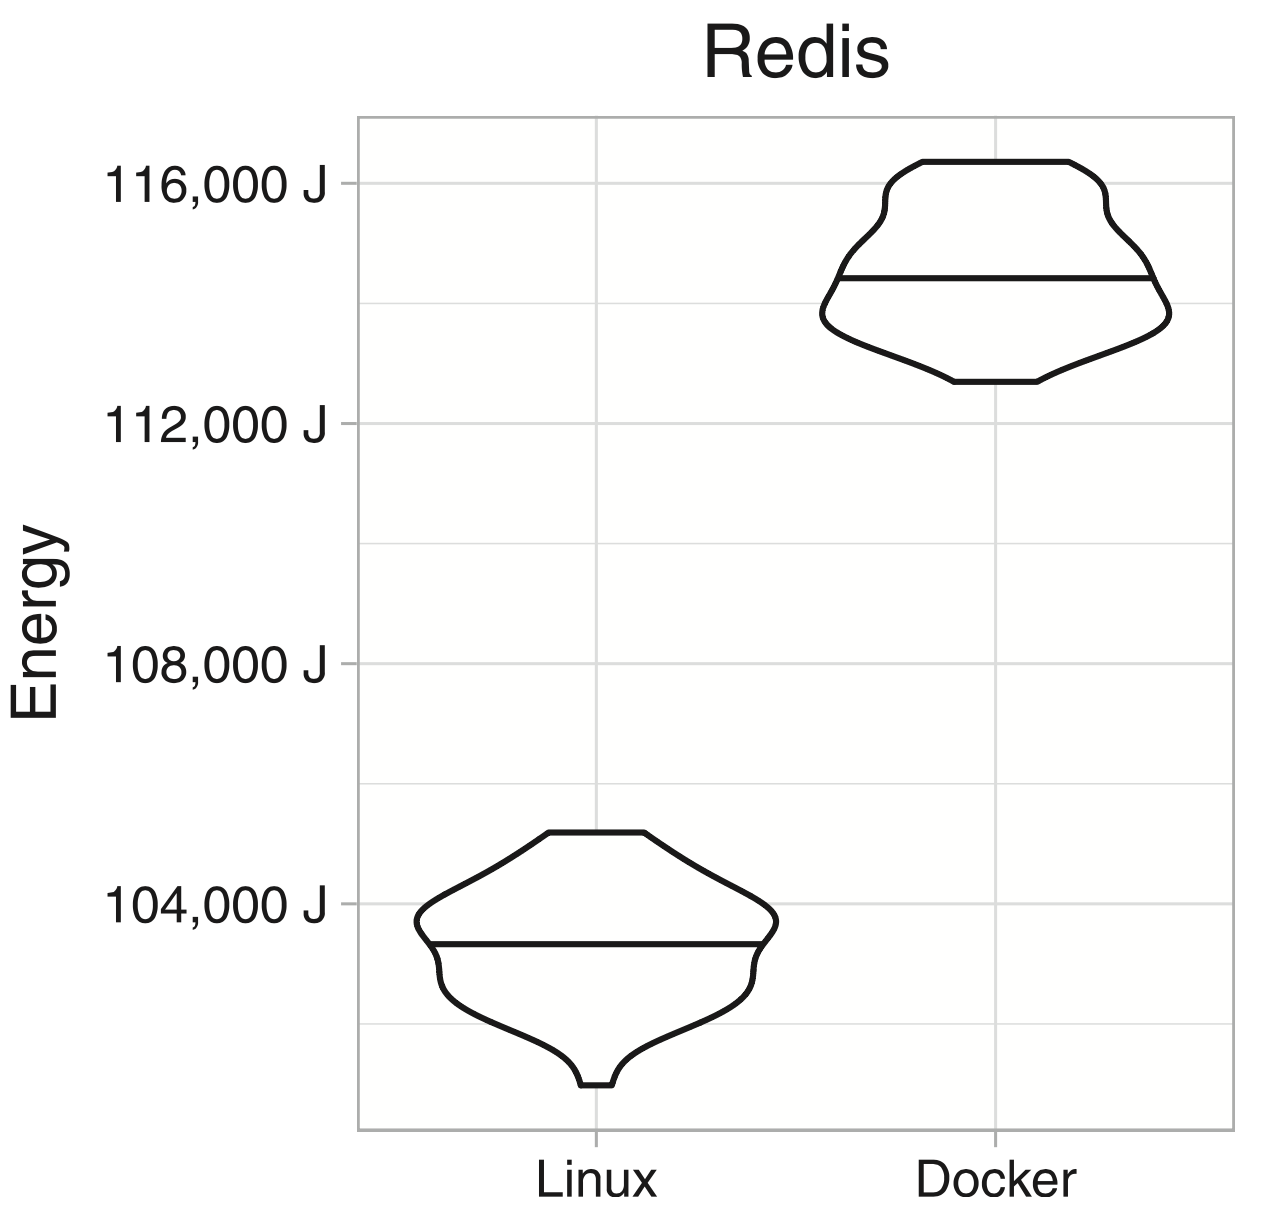
\includegraphics[width=.5\linewidth]{imgs/docker_vs_vm_energy_paper/reddis_energy}
    \caption{execution time and energy consumption of Redis  with and without docker \cite{santos2018does}}\label{fig:docker_reddis}
\end{figure}

%  basically just rephrase the paper 



\subsection{docker and accuracy}
%% TODO : add an introduction, maybe some more details 
And now Since the stat of the art has aggreed on the impact of docker on the energy consumption,Let's discuss it's impact on the accuracy. In other words\\
\textbf{RQ :} does Docker affect the energy variation of the exepements ?

To Answer this question we have conducted a preliminary experiment by running the same benchmarks \textsf{LU}, \textsf{CG} and \textsf{EP} in a Docker container and a flat binary format on 3 nodes of the cluster \textsf{Dahu} to assess if Docker induces an additional variation.
Figure~\ref{fig:docker} reports that this is not the case, as the energy consumption variation does not get noticeably affected by Docker while running a same compiled version of the benchmarks at 5\,\%, 50\,\% and 100\,\% workloads.
In fact, while Docker increases the energy consumption due to the extra layer it implements~\cite{eddie_antonio_santos_how}, it does not noticeably affect the energy variation.
The \emph{standard deviation} (STD) is even slightly smaller ($STD_{Docker}=192 mJ$,$STD_{Binary}=207 mJ$), taking into account the measurements errors and the OS activity.

\begin{figure}
    \center{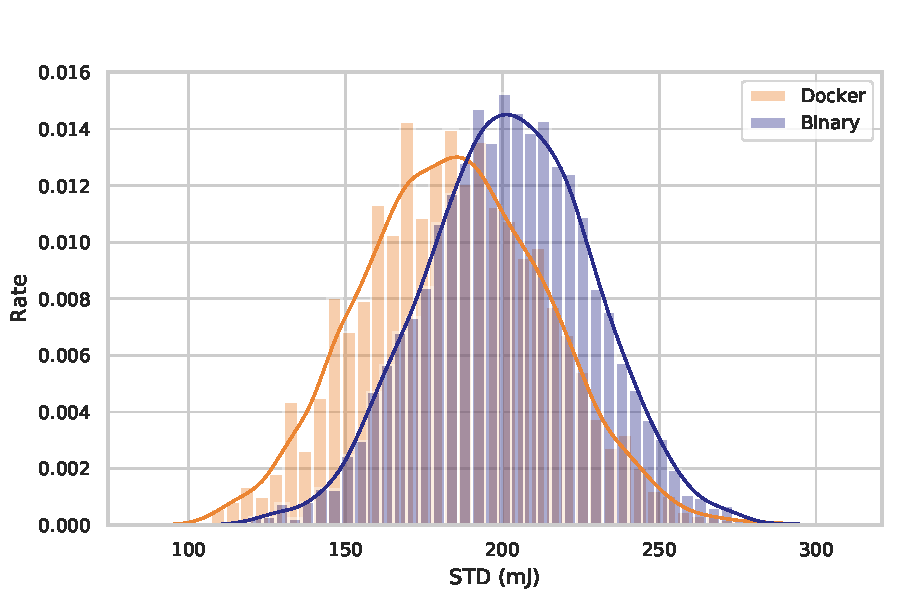
\includegraphics[width=.9\linewidth]{imgs/docvsbin}}
    \caption{Comparing the variation of binary and Docker versions of aggregated \textsf{LU}, \textsf{CG} and \textsf{EP} benchmarks}\label{fig:docker}
\end{figure}